%! Author = kouro
%! Date = 14/01/2024
\documentclass[french,a4paper]{article}
\setcounter{tocdepth}{4}
\setcounter{secnumdepth}{4}
\usepackage{float}
\usepackage{graphicx}
\usepackage{hyperref}
\usepackage{pdfpages}
\usepackage[utf8]{inputenc}
\usepackage[T1]{fontenc}
\usepackage{babel}
\usepackage{tikz}
\usepackage{listings}
\usepackage{xcolor}
\usepackage{booktabs}

\usetikzlibrary{graphs,graphs.standard,arrows,shapes.multipart,chains,positioning,quotes}
\renewcommand{\contentsname}{Table des matières}
\newcommand{\tabitem}{\textbullet~~}
\newcommand{\HRule}{\rule{\linewidth}{0.5mm}}
\usepackage{multirow}
\graphicspath{{img/}}
\title{Projet de compilation}
\usepackage[bottom=2.5cm,top=2.5cm,left=2.5cm,right=2.5cm]{geometry}
\usepackage{textcomp}
\usepackage{amsmath}
\usepackage{amstex}
\setcounter{MaxMatrixCols}{20}
\author{Noé Steiner - Alexis Marcel - Lucas Laurent}
\date{24 Mai 2023}
\lstset{
    language=C,                % choose the language of the code
    numbers=left,              % where to put the line-numbers
    stepnumber=1,              % the step between two line-numbers.
    numbersep=10pt,            % how far the line-numbers are from the code
    tabsize=2,                 % tab size
    showspaces=false,          % show spaces adding particular underscores
    showstringspaces=false,    % underline spaces within strings
    breaklines=true,           % sets automatic line breaking
    frame=single,              % adds a frame around the code
    rulecolor=\color{black},
    basicstyle=\ttfamily\small,
    keywordstyle=\color{blue},
    stringstyle=\color{red},
    commentstyle=\color{green},
    morecomment=[l][\color{magenta}]{\#},
    extendedchars=true,        % lets you use non-ASCII characters; for 8-bits encodings only, does not work with UTF-8
    captionpos=b,              % sets the caption-position to bottom
}

\begin{document}

%\maketitle

    \begin{titlepage}
        \begin{center}

            
\includegraphics[width=0.5\textwidth]{tele_univ}

            \textsc{\Large Rapport final de Projet de compilation}\\[1.5cm]

            \HRule \\[0.4cm]
            { \huge \bfseries Développement d'un compilateur pour le language CanAda\\[0.4cm] }

            \HRule \\[2cm]

            \begin{minipage}{0.4\textwidth}
                \begin{flushleft} \large
                Alexis MARCEL\\
                Lucas LAURENT\\
                Noé STEINER\\
                \end{flushleft}
            \end{minipage}
            \begin{minipage}{0.4\textwidth}
                \begin{flushright} \large
                \emph{Responsable du module :}\\
                M. Olivier FESTOR\\
                Mme. Suzanne COLLIN\\
                \end{flushright}
            \end{minipage}

            \vfill

            {\large 15 Janvier 2024}

        \end{center}
    \end{titlepage}
    \newpage
    \tableofcontents
    \newpage
    \section{Contexte du projet}\label{sec:contexte-du-projet}
    Ce rapport présente le projet réalisé dans le cadre du module PCL1 de la première année du cycle ingénieur à TELECOM Nancy. L'objectif principal est de développer, en groupe, un compilateur pour le langage "canAda", une version simplifiée d'Ada. Ce projet est une opportunité d'approfondir nos compétences en analyse lexicale et syntaxique ainsi que la construction d'un arbre abstrait.

    \section{Introduction}\label{sec:introduction}
    Dans le cadre de nos études, la compréhension et le développement de compilateurs se révèlent cruciaux car ils permettent de mieux comprendre les principes fondamentaux de l'informatique, comme la structure des langages de programmation, l'analyse syntaxique ou encore les arbres abstraits. Cette connaissance est essentielle pour optimiser les performances des programmes, assurer leur sécurité, et développer des logiciels fiables et efficaces. Le projet "canAda" s'inspire d'Ada, un langage connu pour sa fiabilité et sa sécurité. Ce travail nous plonge dans la complexité de la compilation, nous préparant à des applications concrètes dans divers secteurs tels que les systèmes embarqués, la défense, ou l'aéronautique. En développant un compilateur pour "canAda", nous affrontons non seulement les défis techniques relatifs à la conception d'un tel compilateur mais aussi nous nous créons une base de connaissances fondamentale pour nous, futurs ingénieurs.
    Nous avons pris comme décision de faire ce projet en Java car nous avions envie d'approfondir notre connaissance de ce langage et de ses outils.

    \section{Grammaire}\label{sec:grammaire}

    \subsection{Présentation}\label{subsec:presentation}
    Le sujet nous a fourni une grammaire associée au langage "canAda". Cette grammaire est une version simplifiée de la grammaire du langage Ada et était sous une forme abstraire avec notamment des regex.

    \begin{figure}[H]
        \centering
        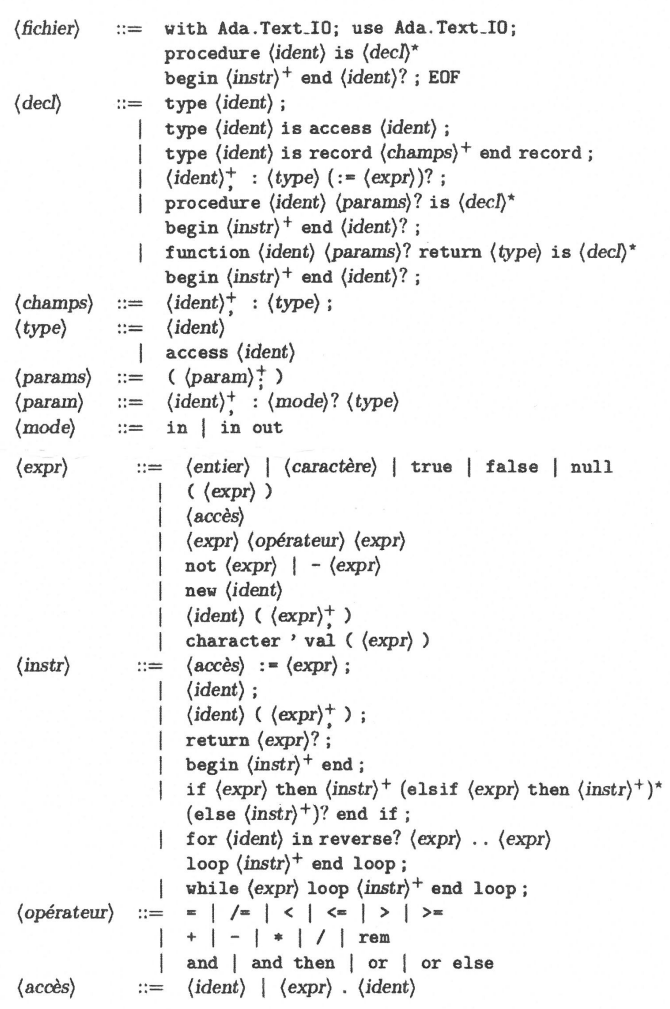
\includegraphics[width=0.8\textwidth]{grammaire_init}
        \caption{Grammaire initiale du Sujet}\label{fig:figure}
    \end{figure}

    \subsection{Étapes de Transformation de la Grammaire}\label{subsec:etapes-de-transformation-de-la-grammaire}

    \subsection{Grammaire Originale en BNF}\label{subsec:grammaire-originale-en-bnf}

    La grammaire initiale du langage "canAda", avant sa transformation en grammaire LL(1), se présente comme suit en BNF sans les regex:

    \begin{verbatim}
        fichier -> with Ada.Text_IO ; use Ada.Text_IO ;
                   procedure ident is <decls> begin <instrs> end <hasident> ; EOF

        decl -> type ident ;
               | type ident is access ident ;
               | type ident is record <champs> end record ;
               | <identsep> : <type> <typexpr> ;
               | procedure ident <hasparams> is <decls> begin <instrs> end <hasident> ;
               | function ident <hasparams> return <type> is <decls> begin <instrs> end <hasident> ;

        decls -> <decl> <decls>
                | ε

        hasident -> ident
                   | ε

        identsep -> ident , <identsep>
                   | ident

        champ -> <identsep> : <type> ;

        champs -> <champ> <champs>
                 | <champ>

        type -> ident
               | access ident

        params -> ( <paramsep> )

        hasparams -> <params>
                    | ε

        paramsep -> <param> ; <paramsep>
                   | <param>

        typexpr -> := <expr>
                  | ε

        param -> <identsep> : <mode> <type>

        mode -> in
               | in out
               | ε

        expr -> entier
               | caractère
               | true
               | false
               | null
               | ( <expr> )
               | <accès>
               | <expr> <opérateur> <expr>
               | not <expr>
               | - <expr>
               | new ident
               | ident ( <exprsep> )
               | character ' val ( <expr> )

        exprsep -> <expr> , <exprsep>
                  | <expr>

        hasexpr -> <expr>
                  | ε

        instr -> <accès> := <expr> ;
                 | ident ;
                 | ident ( <exprsep> ) ;
                 | return <hasexpr> ;
                 | begin <instrs> end ;
                 | if <expr> then <instrs> <elsif> <else> end if ;
                 | for ident in <hasreverse> <expr> .. <expr> loop <instrs> end loop ;
                 | while <expr> loop <instrs> end loop ;

        elsif -> elsif <expr> then <instrs> <elsif>
                 | ε

        else -> else <instrs>
                 | ε

        hasreverse -> reverse
                      | ε

        instrs -> <instr> <instrs>
                  | <instr>

        opérateur -> = | /= | < | <= | > | >= | + | - | * | / | rem | and | and then | or | or else

        accès -> ident
                | <expr> . ident

    \end{verbatim}

    \subsubsection{Élimination de la Récursivité à Gauche}
    La grammaire initiale comportait plusieurs instances de récursivité à gauche. Par exemple, la règle:
    \begin{verbatim}
        expr -> <accès>
        accès -> ident | <expr> . ident
    \end{verbatim}
    a été transformée en:
    \begin{verbatim}
        expr -> ident primary2
        primary2 -> ( exprsep ) acces | acces
        acces -> . ident acces | ε
    \end{verbatim}
    Cette modification élimine la (double ici) récursivité à gauche, rendant la grammaire adaptée pour une analyse LL(1).
    Une autre récursivité à gauche a été supprimé mais elle a été faite aussi à travers la priorisation des règles.

    \subsubsection{Factorisation à Gauche}
    La factorisation à gauche a été nécessaire pour certaines règles. Par exemple:
    \begin{verbatim}
        exprsep -> <expr> , <exprsep>
        exprsep -> <expr>
    \end{verbatim}
    a été réécrite en:
    \begin{verbatim}
        exprsep -> <expr> exprsep'
        exprsep' -> , <expr> exprsep' | ε
    \end{verbatim}
    Ceci assure que la règle peut être analysée de manière déterministe en LL(1).

    \subsubsection{Gestion des Priorités de Calculs}
    Pour gérer correctement les priorités des opérations, la grammaire a été ajustée. Par exemple, les opérations de multiplication et division ont été séparées des opérations d'addition et de soustraction pour respecter leur priorité:
    \begin{verbatim}
        expr -> <expr> <opérateur> <expr>
    \end{verbatim}
    a été réécrite en:
    \begin{verbatim}
        expr -> or_expr
        or_expr -> and_expr or_expr'
        or_expr' -> or or_expr'2 | ε
        or_expr'2 -> and_expr or_expr'
        or_expr'2 -> else and_expr or_expr'
        and_expr -> not_expr and_expr'
        \end{verbatim}
    [\dots]
    \begin{verbatim}
        unary_expr -> - unary_expr
        unary_expr -> primary
        primary -> entier
        primary -> caractère
        primary -> true
        primary -> false
        primary -> null
        primary -> ( expr )
        primary -> ident primary2
        primary -> new ident
        primary -> character ' val ( expr )
    \end{verbatim}
    Cela permet de respecter la hiérarchie des opérations dans les expressions arithmétiques.

    Les ensembles de sélection distincts ont été calculés pour assurer une sélection univoque lors de l'analyse.

    Ces étapes illustrent comment la grammaire initiale a été transformée en une grammaire LL(1), adaptée pour une analyse syntaxique efficace et précise du langage "canAda".

    \subsection{Grammaire Transformée en LL(1)}\label{subsec:grammaire-transformee-en-ll(1)}
    La grammaire transformée en LL(1) se présente comme suit:
    \begin{verbatim}
        fichier -> withAda.Text_IO;useAda.Text_IO; procedure ident is decls begin instrs end hasident ; EOF
        decl -> type ident hasischoose ;
        decl -> identsep : type_n typexpr ;
        decl -> procedure ident hasparams is decls begin instrs end hasident ;
        decl -> function ident hasparams return type_n is decls begin instrs end hasident ;

        hasischoose -> is accorrec | ε

        accorrec -> access ident
        accorrec -> record champs end record

        decls -> decl decls
        decls -> ε

        hasident -> ident
        hasident -> ε

        identsep -> ident identsep2

        identsep2 -> , identsep
        identsep2 -> ε

        champ -> identsep : type_n ;

        champs -> champ champs2

        champs2 -> champs | ε

        type_n -> ident
        type_n -> access ident

        params -> ( paramsep )

        hasparams -> params
        hasparams -> ε

        paramsep -> param paramsep2

        paramsep2 -> ; paramsep
        paramsep2 -> ε

        typexpr -> := expr
        typexpr -> ε

        param -> identsep : mode type_n

        mode -> in modeout
        mode -> ε

        modeout -> out
        modeout -> ε

        expr -> or_expr

        or_expr -> and_expr or_expr'

        or_expr' -> or or_expr'2
        or_expr' -> ε

        or_expr'2 -> and_expr or_expr'
        or_expr'2 -> else and_expr or_expr'

        and_expr -> not_expr and_expr'

        and_expr' -> and and_expr'2
        and_expr' -> ε

        and_expr'2 -> not_expr and_expr'
        and_expr'2 -> then not_expr and_expr'

        not_expr -> equality_expr not_expr'

        not_expr' -> not equality_expr not_expr'
        not_expr' -> ε

        equality_expr -> relational_expr equality_expr'

        equality_expr' -> = relational_expr equality_expr'
        equality_expr' -> /= relational_expr equality_expr'
        equality_expr' -> ε

        relational_expr -> additive_expr relational_expr'

        relational_expr' -> < additive_expr relational_expr'
        relational_expr' -> <= additive_expr relational_expr'
        relational_expr' -> > additive_expr relational_expr'
        relational_expr' -> >= additive_expr relational_expr'
        relational_expr' -> ε

        additive_expr -> multiplicative_expr additive_expr'

        additive_expr' -> + multiplicative_expr additive_expr'
        additive_expr' -> - multiplicative_expr additive_expr'
        additive_expr' -> ε

        multiplicative_expr -> unary_expr multiplicative_expr'

        multiplicative_expr' -> * unary_expr multiplicative_expr'
        multiplicative_expr' -> / unary_expr multiplicative_expr'
        multiplicative_expr' -> rem unary_expr multiplicative_expr'
        multiplicative_expr' -> ε

        unary_expr -> - unary_expr
        unary_expr -> primary

        primary -> entier
        primary -> caractère
        primary -> true
        primary -> false
        primary -> null
        primary -> ( expr )
        primary -> ident primary2
        primary -> new ident
        primary -> character ' val ( expr )

        primary2 -> ( exprsep ) acces
        primary2 -> acces

        exprsep -> expr exprsep2

        exprsep2 -> , exprsep
        exprsep2 -> ε

        hasexpr -> expr
        hasexpr -> ε

        instr -> ident instr2
        instr -> return hasexpr ;
        instr -> begin instrs end ;
        instr -> if expr then instrs elifn elsen end if ;
        instr -> for ident in hasreverse expr .. expr loop instrs end loop ;
        instr -> while expr loop instrs end loop ;

        instr2 -> instr3 := expr ;
        instr2 -> ( exprsep ) instr3 hasassign ;
        instr2 -> ;

        instr3 -> . ident instr3
        instr3 -> ε

        hasassign -> := expr
        hasassign -> ε

        elifn -> elif expr then instrs elifn
        elifn -> ε

        elsen -> else instrs
        elsen -> ε

        hasreverse -> reverse
        hasreverse -> ε

        instrs -> instr instrs2

        instrs2 -> instr instrs2
        instrs2 -> ε

        acces -> . ident acces
        acces -> ε
    \end{verbatim}

    \subsection{Table LL(1)}\label{subsec:table-ll(1)}

    \begin{figure}[H]
        \centering
        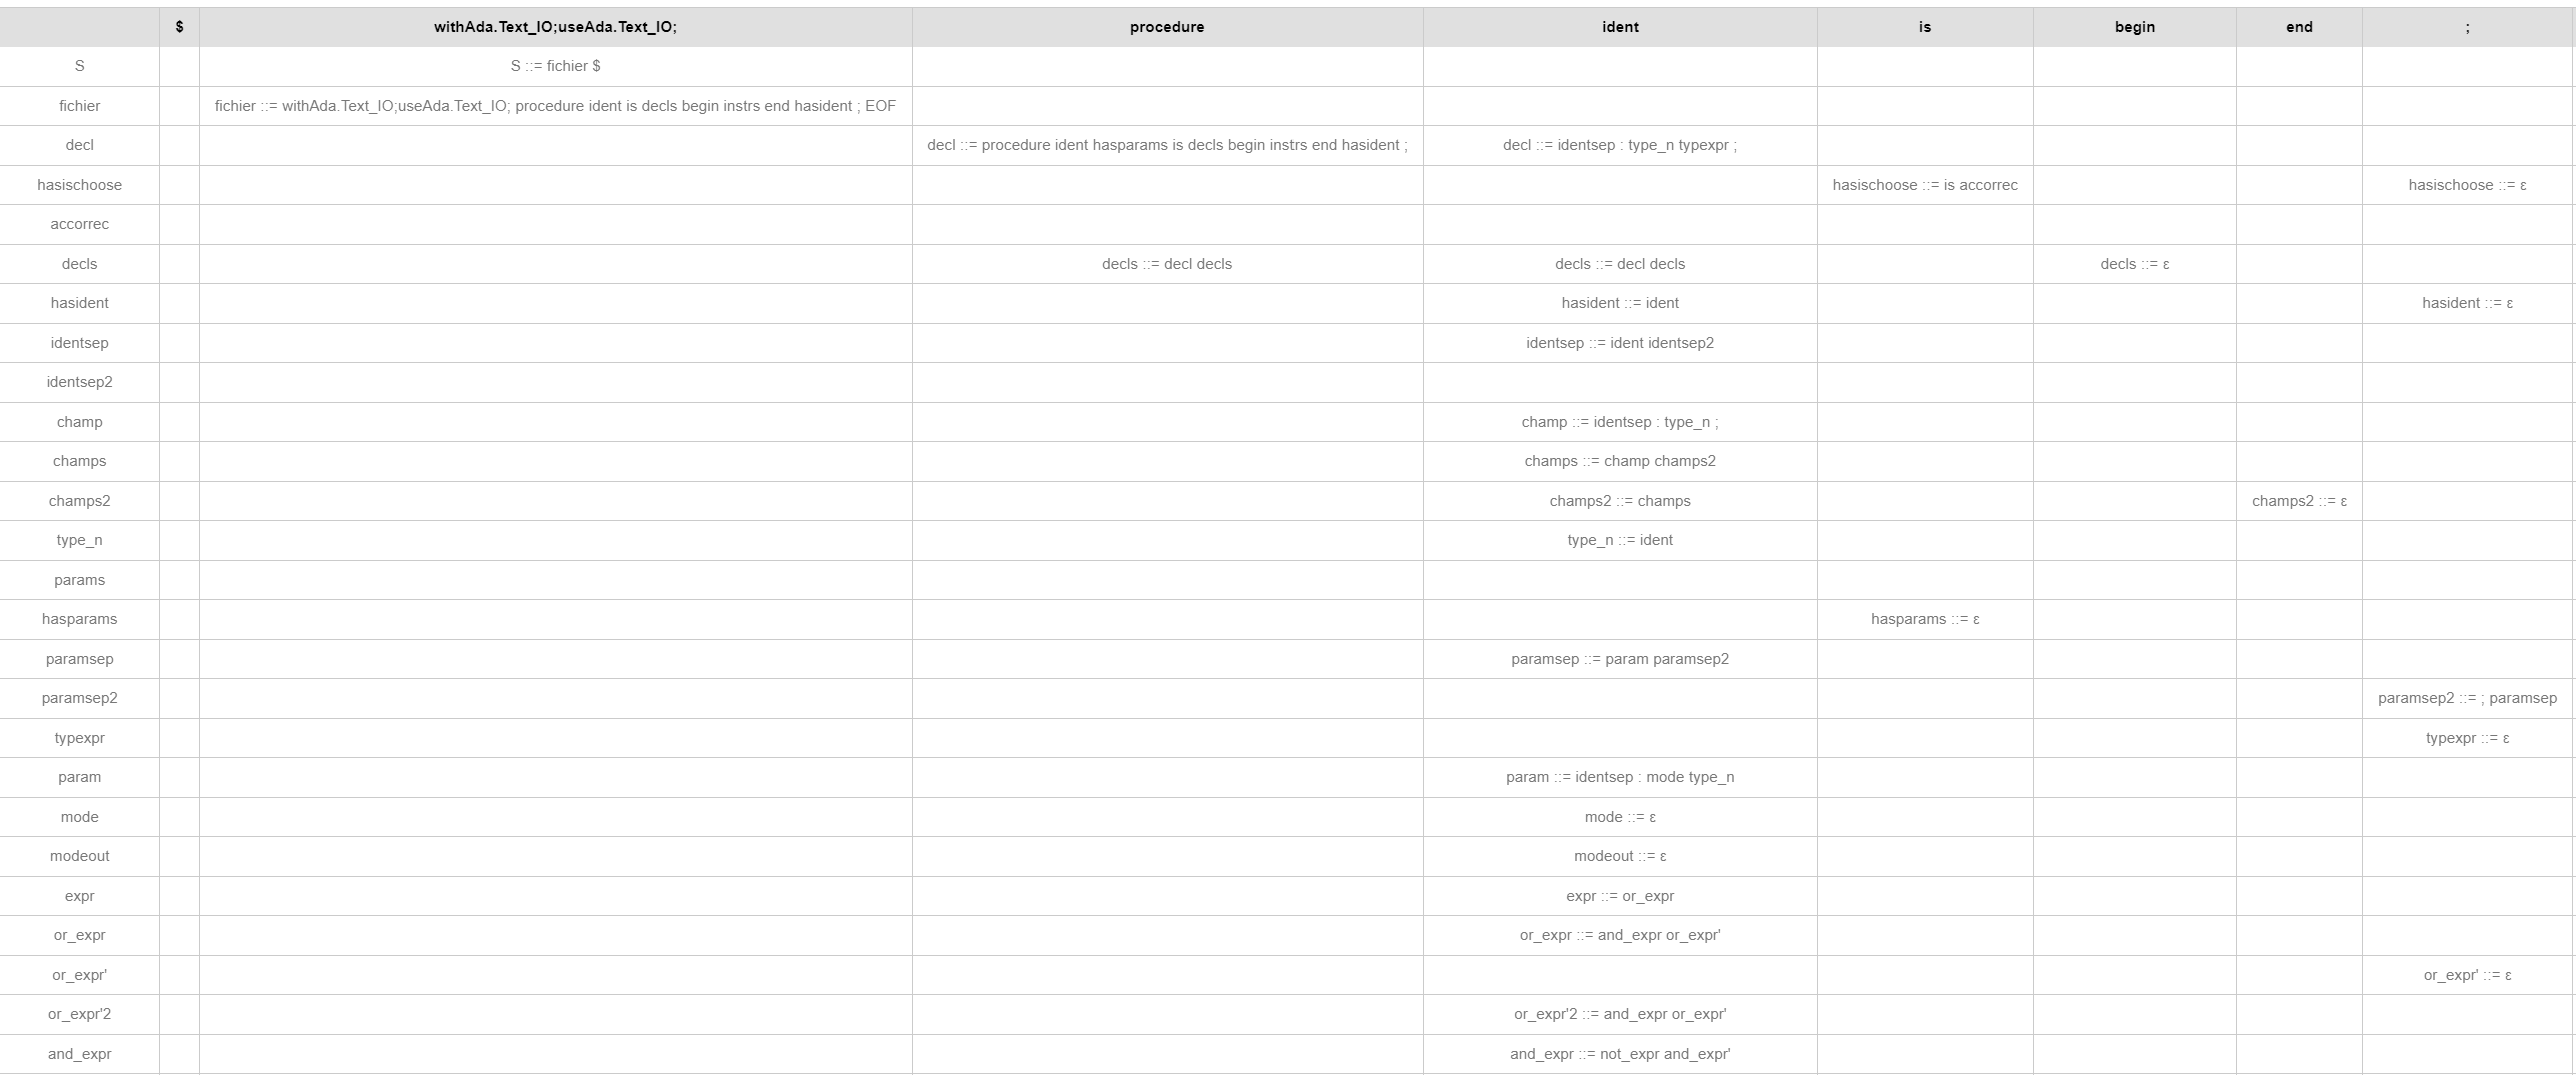
\includegraphics[width=0.8\textwidth]{partial_table}
        \caption{Table LL(1)}\label{fig:figure2}
    \end{figure}

    \section{Analyse Lexicale pour canAda}\label{sec:analyse-lexicale-pour-canada}

    L'analyse lexicale, une étape cruciale dans le processus de compilation, est gérée par notre classe `Lexer`. Cette classe est responsable de la conversion du code source en une série de tokens, facilitant ainsi l'analyse syntaxique ultérieure.

    \subsection{Structure et Fonctionnement du Lexer}\label{subsec:structure-et-fonctionnement-du-lexer}

    La classe `Lexer` lit le code source et identifie les différents tokens en se basant sur un ensemble de règles prédéfinies. Chaque token est une instance de la classe `Token`, qui contient des informations telles que le type de token et la valeur lexicale associée.

    \subsection{Gestion des Tokens}\label{subsec:gestion-des-tokens}

    Des classes spécifiques, comme `Tag` et `PeekingReader`, sont utilisées pour catégoriser les tokens et gérer efficacement la lecture en avance du code source. La classe `Tag` définit les différents types de tokens, tandis que `PeekingReader` permet de lire en avance dans le flux de caractères pour identifier correctement les tokens complexes.

    \subsection{Optimisation et Fiabilité}\label{subsec:optimisation-et-fiabilite}

    Le `Lexer` est conçu pour être à la fois rapide et fiable, capable d'identifier précisément les tokens même dans des cas de syntaxe complexe. Cette précision est essentielle pour garantir une analyse syntaxique sans erreur dans les étapes suivantes du processus de compilation.

    \section{Analyse Syntaxique}\label{sec:analyse-syntaxique}

    La classe `Parser` a été conçue pour analyser les programmes écrits dans le langage "canAda". Chaque méthode de cette classe correspond à un non-terminal de la grammaire LL(1) et est responsable de l'analyse d'une structure syntaxique spécifique du langage.

    \subsection{Structure et Fonctionnement}\label{subsec:structure-et-fonctionnement}

    Dans notre `Parser`, chaque fonction représente un non-terminal de la grammaire. Par exemple, une méthode `expr()` est utilisée pour analyser les expressions, correspondant au non-terminal `expr` de la grammaire. Ces méthodes sont appelées récursivement pour construire l'arbre syntaxique du programme source.

    \subsection{Interaction avec l'Analyseur Lexical}\label{subsec:interaction-avec-l'analyseur-lexical}

    Le `Parser` interagit étroitement avec l'analyseur lexical, recevant un flux de tokens qui sont analysés selon les règles de la grammaire. Cette interaction est cruciale pour la décomposition correcte du programme source en ses composants syntaxiques.

    \subsection{Gestion des Erreurs Syntaxiques}\label{subsec:gestion-des-erreurs-syntaxiques}

    Un aspect essentiel du `Parser` est sa capacité à gérer les erreurs syntaxiques. Lorsque le programme source ne respecte pas les règles de la grammaire, des messages d'erreur descriptifs sont générés, facilitant la localisation et la correction des erreurs par les développeurs. On a notamment appliqué le "panic mode" pour gérer les erreurs syntaxiques. Le Parser continue à analyser le programme source jusqu'à la fin tout en indiquant les erreurs rencontrées.

    \section{Construction de l'Arbre Abstrait Syntaxique pour canAda}\label{sec:construction-de-l'arbre-abstrait-syntaxique-pour-canada}

    La construction de l'arbre abstrait syntaxique (AST) est une étape essentielle du processus de compilation du langage "canAda". L'AST représente la structure syntaxique du programme source d'une manière qui est à la fois concise et facile à manipuler pour les étapes suivantes de la compilation.

    \subsection{Structure et Fonctionnement de l'AST}\label{subsec:structure-et-fonctionnement-de-l'ast}

    Notre système d'AST est construit autour de la classe `ASTNode`, qui sert de classe de base pour les différents types de nœuds de l'arbre. Chaque nœud spécifique, comme `OperatorNode`, `ParameterNode`, ou `ProgramNode`, hérite de `ASTNode` et représente une construction syntaxique spécifique du langage.

    \subsection{Représentation des Structures Syntaxiques}\label{subsec:representation-des-structures-syntaxiques}

    Les nœuds de l'AST capturent les éléments essentiels des structures syntaxiques du programme, comme les opérations, les paramètres, et la structure globale du programme. Par exemple, `OperatorNode` représente une opération arithmétique ou logique, tandis que `ProgramNode` représente la structure globale du programme canAda.

    \subsection{Rôle dans le Processus de Compilation}\label{subsec:role-dans-le-processus-de-compilation}

    L'AST joue un rôle central dans le processus de compilation. Après l'analyse syntaxique, le programme source est transformé en un AST, qui est ensuite utilisé pour les étapes de vérification sémantique, d'optimisation, et de génération de code. Cette représentation permet une manipulation plus aisée et plus efficace du programme source.

    \section{Tests et Validation}\label{sec:tests-et-validation}


    \section{Gestion de projet}\label{sec:gestion-de-projet}

    \subsection{Équipe de projet}\label{subsec:equipe-de-projet}
    Ce projet est un projet local réalisé en groupe de 3 personnes~:
    \begin{itemize}
        \item Alexis MARCEL
        \item Lucas LAURENT
        \item Noé STEINER
    \end{itemize}

    \subsection{Organisation au sein de l’équipe projet}\label{subsec:organisation-au-sein-de-lequipe-projet}
    Nous avons réalisé plusieurs réunions, en présentiel dans les locaux de Télécom Nancy mais la plupart de notre collaboration a eu lieu sur Discord. Ces réunions nous ont permis de mettre en commun nos avancées régulièrement, de partager nos connaissances sur des problématiques et de nous organiser de manière optimale.
    En plus des réunions d'avancement régulières, nous avons également réalisé des réunions techniques afin de résoudre un problème ou bien de réfléchir à la conception.

    Ensuite, nous avons utilisé GitLab pour gérer les différentes versions du développement de notre application, ainsi que les différentes
    branches nous permettant de travailler simultanément sans conflit.

    \subsection{Matrice RACI}\label{subsec:matrice-raci}
    Nous avons choisi de ne pas faire de matrice RACI à cause des choix d'organisation que nous avons faits. En effet,
    nous avons décidé de travailler en groupe sur toutes les tâches, ce qui fait que nous sommes tous responsables de toutes les tâches et qu'il n'y a, de ce fait,
    pas de répartition précise des tâches.

    \begin{figure}[H]
        \centering
        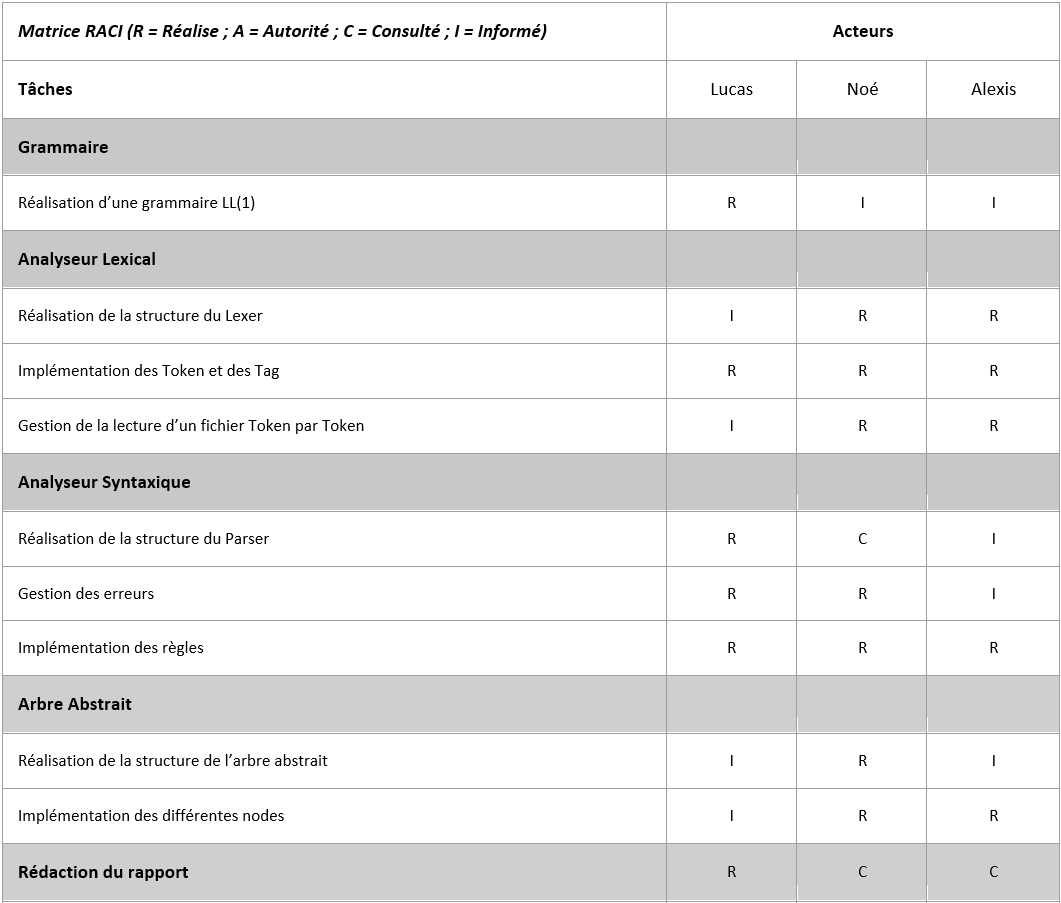
\includegraphics[width=1\textwidth]{RACI}
        \caption{Matrice RACI}\label{fig:figure3}
    \end{figure}

    \subsection{Répartition du Temps de Travail sur le Projet}\label{subsec:repartition-du-temps-de-travail-sur-le-projet}

    \begin{tabular}{@{}llll@{}}
        \toprule
        Tâche & Lucas & Noé & Alexis \\ \midrule
        Grammaire & 10h & - & - \\
        Structure du Lexer & - & 2h & 2h \\
        Lecture du fichier (token par token) & - & 7h & 7h \\
        Implémentation des Token et des Tag & 2h & 2h & 2h \\
        Structure du Parser & 2h & - & - \\
        Gestion des erreurs & 4h & 4h & - \\
        Implémentation des règles & 3h & 3h & 3h \\
        Structure de l'arbre abstrait & - & 2h & - \\
        Implémentation des différents nodes & - & 5h & 5h \\
        Rédaction du rapport & 4h & - & - \\
        \midrule
        Total & 25h & 25h & 19h \\ \bottomrule
    \end{tabular}

\section{Conclusion}\label{sec:conclusion}

    Le développement du compilateur pour le langage "canAda" a été une expérience enrichissante et formatrice. À travers les diverses phases du projet, de la conception de la grammaire LL(1) à l'implémentation de l'analyseur lexical et syntaxique, en passant par la construction de l'arbre abstrait syntaxique, chaque membre de l'équipe a contribué de manière significative. Ce projet nous a permis de consolider nos connaissances théoriques en informatique et de développer des compétences pratiques essentielles en matière de compilation. Les défis rencontrés, notamment dans la gestion des erreurs et l'optimisation des performances, ont renforcé notre compréhension des aspects complexes de la conception de compilateurs. Ce projet a non seulement abouti à la création d'un compilateur fonctionnel pour "canAda", mais il a également été une opportunité précieuse d'apprentissage et de collaboration pour notre équipe.
Nous avons pu mettre en pratique les connaissances acquises en cours de PCL1 et nous avons pu approfondir nos connaissances en programmation et en compilation et avons hâte de poursuivre ce projet en PCL2.

\end{document}
